\apendice{Documentación técnica de programación}
\section{Introducción}
En este apéndice se va a describir la documentación técnica de programación, incluyendo la estructura de directorios, manual para el programador, despliegue de herramientas para desarrollo, ejecución del proyecto y pruebas del sistema.

\section{Estructura de directorios}
El proyecto tiene una estructura de directorio tal que:
\begin{itemize}
    \item \textit{./doc/}: Todos los archivos relacionados con la documentación del proyecto.
    \item \textit{./WebRTCGuidesApp/}: Todos los archivos relacionados con la \textit{webapp}.
    \item \textit{./WebRTCGuidesApp/src/}: Todos los archivos relacionados con los componentes de \textit{React}.
    \item \textit{./APIsGateways/openapi-server-container/openapi\_server/}: Todos los archivos relacionados con la \textit{API}.
    \item \textit{./APIsGateways/openapi-server-container/openapi\_server/config/}: Todos los archivos relacionados con la configuración de la API.
    \item \textit{./APIsGateways/openapi-server-container/openapi\_server/controllers/}: Todos los archivos relacionados con los controladores.
    \item \textit{./APIsGateways/openapi-server-container/openapi\_server/models/}: Todos los archivos relacionados con los modelos y esquemas del ORM.
    \item \textit{./APIsGateways/openapi-server-container/openapi\_server/openapi/}: El archivo de extensión \textit{.yaml} que tiene las especificaciones de la \textit{API}.
    \item \textit{./APIsGateways/}: Todos los servicios que funcionan en el mismo \textit{docker-compose}.

\end{itemize}

\section{Manual del programador}
En este apartado se van a explicar los puntos necesarios para que se pueda entender el despliegue de la aplicación para desarrollar sobre ella.

Durante este proyecto se ha trabajado con \textit{Github}, por lo que el repositorio del proyecto está allí, para obtenerlo primero tendríamos que clonar el repositorio:

\subsection{Clonar repositorio}

Antes de nada es necesario tener instalado \textit{Git} en la consola de comandos, ya bien sea en \textit{Windows} o en \textit{Linux} (a veces viene de serie):

\begin{itemize}
    \item 1. Abrir el \textit{bash} de \textit{git}, donde nos interese clonar el repositorio.
    \item 2. Escribir el comando: 
    \item 3. Una vez tenemos el repositorio, podremos acceder y tendremos que cambiar a la rama de \textit{dev} con el comando: \textit{git checkout dev}.
\end{itemize}
\FloatBarrier
\begin{figure}[h]
    \centering
    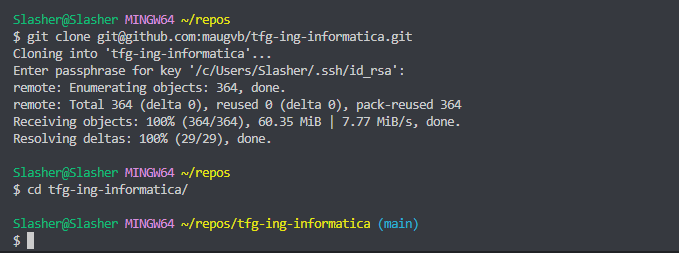
\includegraphics[width=12cm,height=12cm,keepaspectratio]{img/git.png}
    \caption{Clonado de repositorio de la herramienta \textit{Github} desde \textit{WSL 2}.}
    \label{fig:Flujo de navegabilidad de los usuarios por las páginas}
\end{figure}
\FloatBarrier

\subsection{Entorno de desarrollo}
Para el entorno de desarrollo se ha utilizado\textit{\textbf{Visual Studio Code}}.
\begin{itemize}
    \item 1. Si no lo tuviésemos descargado, lo descargaríamos.
    \item 2. Teniendo \textit{WSL 2} en \textit{Windows}, o ejecutando en \textit{Ubuntu}, desde la línea de comandos nos aseguramos que tenemos el comando code instalado.
    \item 3. Desde la consola de comando vamos a la carpeta del proyecto.
    \item 4. Escribimos el siguiente comando: \textit{"code ."}, que abrirá la carpeta del proyecto directamente en la ventana de \textit{Visual Studio Code}.

\end{itemize}
\section{Compilación, instalación y ejecución del proyecto}
En este apartado se explicará el despliegue de la aplicación.
\subsection{Compilación}
En este subapartado nos centraremos en la compilación de nuestro proyecto.
\begin{itemize}
    \item \textit{\textbf{Webapp}}: para la compilación del proyecto en modo desarrollador, tendríamos que ir a la carpeta \textit{/WebRTCGuidesApp} y ejecutar el comando \textit{yarn dev}, previamente deberemos de haber lanzado el comando \textit{yarn install} para la instalación de los \textit{node\_modules}, que son las dependencias externas de la aplicación. Después de lanzar el comando \textit{yarn dev} nuestra aplicación compilada estará corriendo en \textit{https://localhost:3000}.
    \item \textit{\textbf{API}}: No es un proceso de compilación, pero si hacemos algún cambio en el código de la \textit{API}, para que se actualicen os cambios en el contenedor, debemos ir a la carpeta \textit{APIsGateway} y lanzar el comando \textit{docker-compose build}.
\end{itemize}
\subsection{Ejecución}
Para la ejecución de los servicios, tenemos un \textit{Makefile} en la raíz del proyecto donde:
\begin{itemize}
    \item Para hacer deploy de la app debemos ejecutar el comando \textit{make run-build}.
    \begin{itemize}
        \item \textit{API} en \textit{http://ip-local:8080}
        \item Web en \textit{https://ip-local:80}
    \end{itemize}
    \item Iniciar servicios en modo \textit{developer} tendremos que ejecutar el comando \textit{make dev}. Donde quedarán activos los servicios:
    \begin{itemize}
        \item \textit{API} en \textit{http://localhost:8080}
    \end{itemize}
    
    \item Para eliminar la base de datos debemos de ejecutar el comando \textit{make clean}.
\end{itemize}
\subsection{Despliegue Hardware en entorno físico}
Para el despliegue en un entrono real debemos:
\begin{itemize}
    \item Cambiar \textit{firmware} de las placas en función de los roles: \textit{Anchors}, \textit{Tags} y \textit{Listeners}.
    \item Colocar los \textit{Anchors} y el \textit{Listener}, y colocarlos en las salas.
    \item Con las coordenadas de los \textit{Anchors} en el mapa y una \textit{Room} dibujada, modificamos el código en la \textit{raspberry} para hacer la traslación. 
    \item Y ya obtendríamos información en la \textit{webapp} de los \textit{Tags}.
\end{itemize}
\section{Pruebas del sistema}
En este proyecto han habido dos tipos de pruebas:
\begin{itemize}
    \item Pruebas generales. Estas pruebas se realizaron a modo de auditorías para comprobar los progresos en la aplicación, pasando en todos los estándares de la empresa.
    \item Prueba de estrés. Prueba en la que se lleva al límite una parte de la aplicación para ver su respuesta.
\end{itemize}
\subsection{Prueba 1}
    En esta prueba se utilizaron una sala especifica de la oficina, donde se colgaron cuadros, con una red de reconocimiento de cuadros, ya entrenada. Además se comprobó la fiabilidad de la localización \textit{indoor} con 3 \textit{Anchors} y 1 \textit{Tag} a modo de usuario.
    
    El usuario lleva una \textit{tablet} con la web funcionando, compartiendo vídeo y audio, y apunta con la cámara a una de las obras de arte, así el guia puede dibujar sobre ella.
\subsection{Prueba 2}
    En esta prueba se utilizaron dos salas especificas de la oficina, donde se colgaron cuadros, con una red de reconocimiento de cuadros, ya entrenada. Además se comprobó la fiabilidad de la localización indoor con 3 \textit{Anchors} por sala y 1 \textit{Tag} a modo de usuario.
    
    El usuario lleva una \textit{tablet} con la web funcionando, compartiendo vídeo y audio, y apunta con la cámara a una de las obras de arte, así el guia puede dibujar sobre ella.
\subsection{Prueba 3}
    En esta prueba se utilizaron una sala especifica de la oficina, donde se colgaron cuadros, con una red de reconocimiento de cuadros, ya entrenada. Además se comprobó la fiabilidad de la localización indoor con 3 \textit{Anchors} y 2 \textit{Tag} a modo de usuario.
    
    Los usuarios llevan una \textit{tablet} con la web funcionando, compartiendo vídeo y audio, y apuntan con la cámara a una de las obras de arte, así el guia puede dibujar sobre ella.

\subsection{Prueba de estrés}
La página de mapa, la \textit{API} y la base de datos, se someten a una prueba de estrés con el \textit{script} en la carpeta \textit{WebRTCGuidesAPP/test/TagsInMap.py}. Cuando se ejecuta añade un \textit{Tag} y un usuario con nombres aleatorios enlazados. Las \textit{Tags} se generan con coordenadas aleatorias dentro de un rango determinado, para poder comprobar el comportamiento del mapa en tiempo real.